%1521001##1##.tex
\documentclass[12pt,letterpaper]{article}
\usepackage{mathptmx}
\usepackage[margin=1in]{geometry}

\usepackage{setspace}
\singlespacing
  
\usepackage{amssymb,latexsym}
\usepackage[round,sort]{natbib}
\usepackage{fancyhdr}
\usepackage{lastpage}
\usepackage{graphicx,multirow}
\graphicspath{ {qe1/} }

% Bold Table and Figure captions
\usepackage{caption}
\captionsetup{figurename=FIGURE}
\captionsetup{tablename=TABLE}
\captionsetup[figure]{labelfont=bf}
\captionsetup[table]{labelfont=bf}
  
% Turns off all section numbering
\setcounter{secnumdepth}{0} 

  % Places all tables at end of document and creates AOM-style table-here placeholders
  \usepackage[nolists]{endfloat} % Places all figures and charts at end of manuscript and adds 'insert table x about here' lines.
  \renewcommand{\figureplace}{
    \begin{center}
    \begin{singlespace}
    ------------------------------------\\
    Insert \figurename \ \thepostfig\ about here.\\
    ------------------------------------
    \end{singlespace}
    \end{center}}
  \renewcommand{\tableplace}{%
    \begin{center}
    \begin{singlespace}
    ------------------------------------\\
    Insert \tablename \ \theposttbl\ about here.\\
    ------------------------------------
    \end{singlespace}
    \end{center}}

  \usepackage{titlesec}
   \titleformat{\title}
       {\filcenter\normalfont\bfseries\uppercase}{\thetitle}{1em}{}
  \titleformat{\section}
    {\filcenter\normalfont\bfseries\uppercase}{\thesection}{1em}{}
  \titleformat{\subsection}
    {\normalfont\bfseries}{\thesubsection}{1em}{}
  \titleformat{\subsubsection}[runin]
   {\normalfont\bfseries\slshape}{\thesubsubsection}{1em}{\hspace*{\parindent}}
       
\usepackage{tabu}
\usepackage{textcomp}
\usepackage{listings}
\usepackage{hyperref}
\usepackage{verbatim}
\usepackage{tabu}
\hypersetup{
    colorlinks=true,
    linkcolor=blue,
    filecolor=cyan,      
    urlcolor=cyan,
    citecolor=blue,
}

\usepackage{etoolbox}

\makeatletter

% Patch case where name and year are separated by aysep
\patchcmd{\NAT@citex}
  {\@citea\NAT@hyper@{%
     \NAT@nmfmt{\NAT@nm}%
     \hyper@natlinkbreak{\NAT@aysep\NAT@spacechar}{\@citeb\@extra@b@citeb}%
     \NAT@date}}
  {\@citea\NAT@nmfmt{\NAT@nm}%
   \NAT@aysep\NAT@spacechar\NAT@hyper@{\NAT@date}}{}{}

% Patch case where name and year are separated by opening bracket
\patchcmd{\NAT@citex}
  {\@citea\NAT@hyper@{%
     \NAT@nmfmt{\NAT@nm}%
     \hyper@natlinkbreak{\NAT@spacechar\NAT@@open\if*#1*\else#1\NAT@spacechar\fi}%
       {\@citeb\@extra@b@citeb}%
     \NAT@date}}
  {\@citea\NAT@nmfmt{\NAT@nm}%
   \NAT@spacechar\NAT@@open\if*#1*\else#1\NAT@spacechar\fi\NAT@hyper@{\NAT@date}}
  {}{}

\lstset{
basicstyle=\ttfamily,
columns=flexible,
breaklines=true
}
\newenvironment{hypothesis}{
  	\itshape
  	\leftskip=\parindent \rightskip=\parindent
  	\noindent\ignorespaces}

\fancypagestyle{plain}{
  \renewcommand{\headrulewidth}{0pt}
  \fancyhf{}
}	


\begin{document}
\title{Inducing Strategic Initiatives at a Startup Firm:\\Understanding the Role of the Co-founding Team}
\date{}
\maketitle

\begin{abstract} 
\normalsize I propose here, a study to understand the process of inducing strategic initiatives at a startup firm. Building on the model of strategy as a process of guided evolution \citep{Lovas2000}, I seek to detail how co-founders at a startup firm induce strategic initiatives by orchestrating influence on variation, retention and selection of ideas, people and projects over time. Using a comparative case study of Paypal and Billpoint at around the turn of the 20th century, I hope to enrich the \cite{Lovas2000} model in the empirical context of the digital economy.
\end{abstract}


{\textbf{Keywords:} \\\indent co-founders, process model, strategic initiatives, variation selection retention}

\newpage
\pagestyle{fancy}
\fancyhf{}
\lhead{Inducing Strategic Initiatives at a Startup Firm}
\rhead{\thepage}

\begin{center}
\textbf{Inducing Strategic Initiatives at a Startup Firm: Understanding the Role of the Co-founding Team}\vspace{1cm}
\end{center}

\begin{quotation}
\textit{I disagree and commit all the time. We recently greenlit a particular Amazon Studios original. I told the team my view: debatable whether it would be interesting enough, complicated to produce, the business terms aren\textquotesingle t that good, and we have lots of other opportunities. They had a completely different opinion and wanted to go ahead. I wrote back right away with \textbf{``I disagree and commit and hope it becomes the most watched thing we\textquotesingle ve ever made."} Consider how much slower this decision cycle would have been if the team had actually had to convince me rather than simply get my commitment.}\par
\null\hfill \textbf{\textit{Jeff Bezos}}, reflecting on a recent \textit{strategic initiative} at Amazon \citep{Bezos2016}.
\end{quotation}

One of the recent  debates among scholars in the strategy process tradition is  whether strategic initiatives in firms are induced, are autonomous or are both. In incorporating a ``variation selection retention" framework into the process research tradition, \cite{Burgelman1991} presents the strategic process as being either induced by management or being autonomous from across the organization. \cite{Lovas2000} on the other hand conceive of all strategies as being autonomous.\par

\cite{Lovas2000} define strategic initiatives as ``a deliberate effort by a firm at creating or appropriating economic value from the environment, which is organized as an independent project with its own profit and loss responsibility". The focus on economic value leads to the additional recognition that not all strategic initiatives survive the initial stages to become a part of the firm\textquotesingle s product line as the strategic initiative could be hampered by any number of internal, technical or market related issues. This definition lends itself into an evolutionary process model consisting of variation (the introduction of a new product or service), selection (appropriating resources from the environment), and retention (continued capacity to appropriate resources over time). Saliently, this maybe applied to internal as well as external market conditions of a firm. By treating the organization itself as the platform for ecological selection, \cite{Lovas2000} suggest that all strategic processes may either be considered autonomous or induced. \par

The management of strategic initiatives involves selecting and motivating talent, communicating the strategic intent, guiding resource allocation and providing sense and direction when things do not work out. The \cite{Lovas2000} model is particularly appropriate in the context of a startup firm, where traditional management is either absent or is manifested in a decentralized way. If we assume that all strategic initiatives are autonomous, it becomes interesting to understand how startup firms guide the strategic initiatives in the direction of the co-founders\textquotesingle \ strategic intent. As the quote from Jeff Bezos at the beginning of this section suggests, strategic initiatives at firms make take complex paths. This provides the motivation for the study proposed in this paper, to simplify and explain that process better.\par

In the following section, I review process theories of the past and present and suggest why the \cite{Lovas2000} framework may be the appropriate one to study strategic initiatives in a startup firm. In the section following the next, I then propose a comparative case study of PayPal and Billpoint to further our understanding of how strategic initiatives are induced at a startup firm. 

\section{Review of the evolution of the strategy process literature}
The tradition of process research applied to strategic initiatives goes at least as far back as \cite{Bower1970}. I briefly trace the evolution of this tradition in the following sections. A snapshot of the original models have been provided in Appendix A.

\subsection{Classical theories}
\cite{Noda1996} capture the ethos of strategy process researchers by drawing attention to various complexities inherent in organizations. They highlight ``possible goal incongruence", ``information asymmetry", ``organizational politics" \citep{Barnard1938, Simon1997, Cyert1963}, and ``unpredictable and uncontrollable environments" \citep{Schumpeter1934, Nelson1982, Thompson1967, Pfeffer1978} as having driven process researchers to describe how strategy is formed in practice rather than prescribing what it should be \citep{Mintzberg2005}.\par
\cite{Bower1970}\textquotesingle s classic study demonstrated that the role of top managers is limited in that they do not necessarily have the appropriate knowledge or information to evaluate technical and economic aspects of the strategic initiatives, and tend to rely on the track records or credibility of proposing middle managers in making resource allocation decisions. Figure ~\ref{fig:Bower1970} in the appendix displays the original resource allocation process suggested by \cite{Bower1970}. \cite{Mintzberg1978} suggested that strategy is, more or less, emergent from lower levels of organizations  (see Figure ~\ref{fig:Mintzberg1978}). \cite{Quinn1980} suggested strategy emerged incrementally with logical guidance from the top  (see Figure ~\ref{fig:Quinn1980a} and Figure ~\ref{fig:Quinn1980b}). The Bowerian model was further extended by \cite{Burgelman1983b} in his study on internal corporate venturing (ICV) in a large corporation. In summarizing the tradition, \cite{Noda1996} suggest that the Bower-Burgelman (B-B) process model of strategy making in a large, complex firm depicts multiple, simultaneous, interlocking, and sequential managerial activities over three levels of organizational hierarchy (bottom, middle, and top managers) and conceptualizes intraorganizational strategy-making processes as consisting of four subprocesses: two interlocking bottom-up core processes of definition and impetus and two overlaying corporate processes of structural context determination and strategic context determination (see Figure  ~\ref{fig:Burgelman1983b}).

\subsection{Including the Variation Selection Retention framework in the \cite{Burgelman1991, Burgelman1994} Model}

The intraorganizational perspective (see Figure ~\ref{fig:Burgelman1991}) by \cite{Burgelman1991} extended the frameworks presented by \cite{Mintzberg1978} and \cite{Quinn1980} by highlighting  processes through which emergent strategies become part of realized strategies and by providing some evidence that logical incrementalism is likely to be variation reducing. 

\begin{figure}[h]
\begin{centering}
  \caption{Intraorganizational Ecology of Strategy Making and Organizational Adaptation, adopted from \cite{Burgelman1991}}
  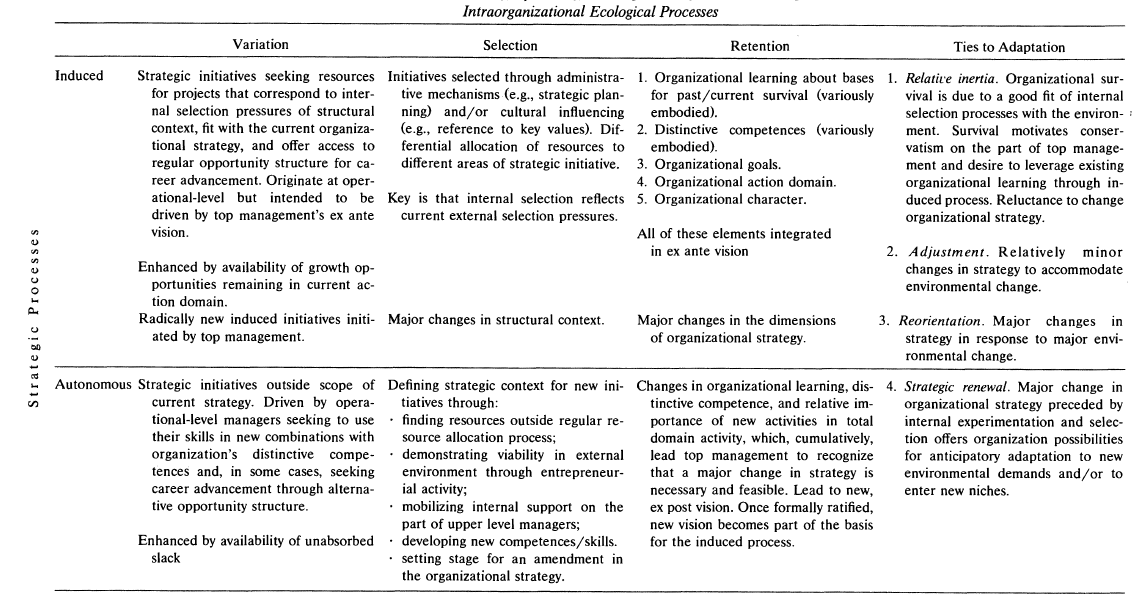
\includegraphics[width=\textwidth]{Burgelman1991}
  \label{fig:Burgelman1991}
\end{centering}
\end{figure}

Burgelman (through \cite{Burgelman1991, Burgelman1994} introduced into this tradition the variation selection retention framework (see Figure ~\ref{fig:Burgelman1994}) from the literature on organizational evolution and ecology \citep{Campbell1965, Nelson1982}. This model suggests that autonomous strategic initiatives serve to challenge the formal strategy of the firm. The key task of top management in this model is to therefore resolve the tension between the autonomous and induced strategy processes by acting as the selection filter through resource allocation decisions.

\begin{figure}[h]
\begin{centering}
  \caption{Forces driving the strategic business-exit process, adopted from \cite{Burgelman1994}}
  \includegraphics[width=\textwidth]{Burgelman1994}
  \label{fig:Burgelman1994}
\end{centering}
\end{figure}

\subsection{Treating all strategic processes as autonomous/induced in the \cite{Lovas2000} Model}
In contrast to the Burgelman view described above, \cite{Lovas2000} describe guided evolution as being based on the experiences of a firm that has attempted to replicate a natural selection environment within itself (see Figure ~\ref{fig:Lovas2000a}). They argue therefore that all strategic initiatives may be seen as being autonomous in the sense that someone in the organization initiates them. Yet, they may all be seen as being induced in the sense that the process of variation selection retention is guided by a strategic intent that is defined by top management. As a result of this difference, guided evolution posits a role of top management that is very different from the role one can infer from Burgelman's model. Relative to the \cite{Burgelman1991} model, the \cite{Lovas2000} model  (see Figure ~\ref{fig:Lovas2000b}) suggests that top management\textquotesingle s role in shaping the strategic context maybe be retroactive rationalization and their influence on structural context  severely constrained. The role of top management in this model to create an administrative systems to replicate the processes of natural selection within the organization and to guide those processes by defining the strategic intent, strategic initiatives and human and social capital. 

\begin{figure}[h]
\begin{centering}
  \caption{The five elements of guided evolution, adopted from \cite{Lovas2000}}
  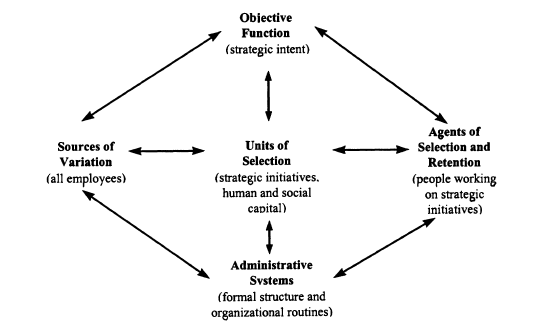
\includegraphics[width=\textwidth]{Lovas2000a}
  \label{fig:Lovas2000a}
\end{centering}
\end{figure}

\begin{figure}[h]
\begin{centering}
  \caption{A model of strategic management as guided evolution, adopted from \cite{Lovas2000}}
  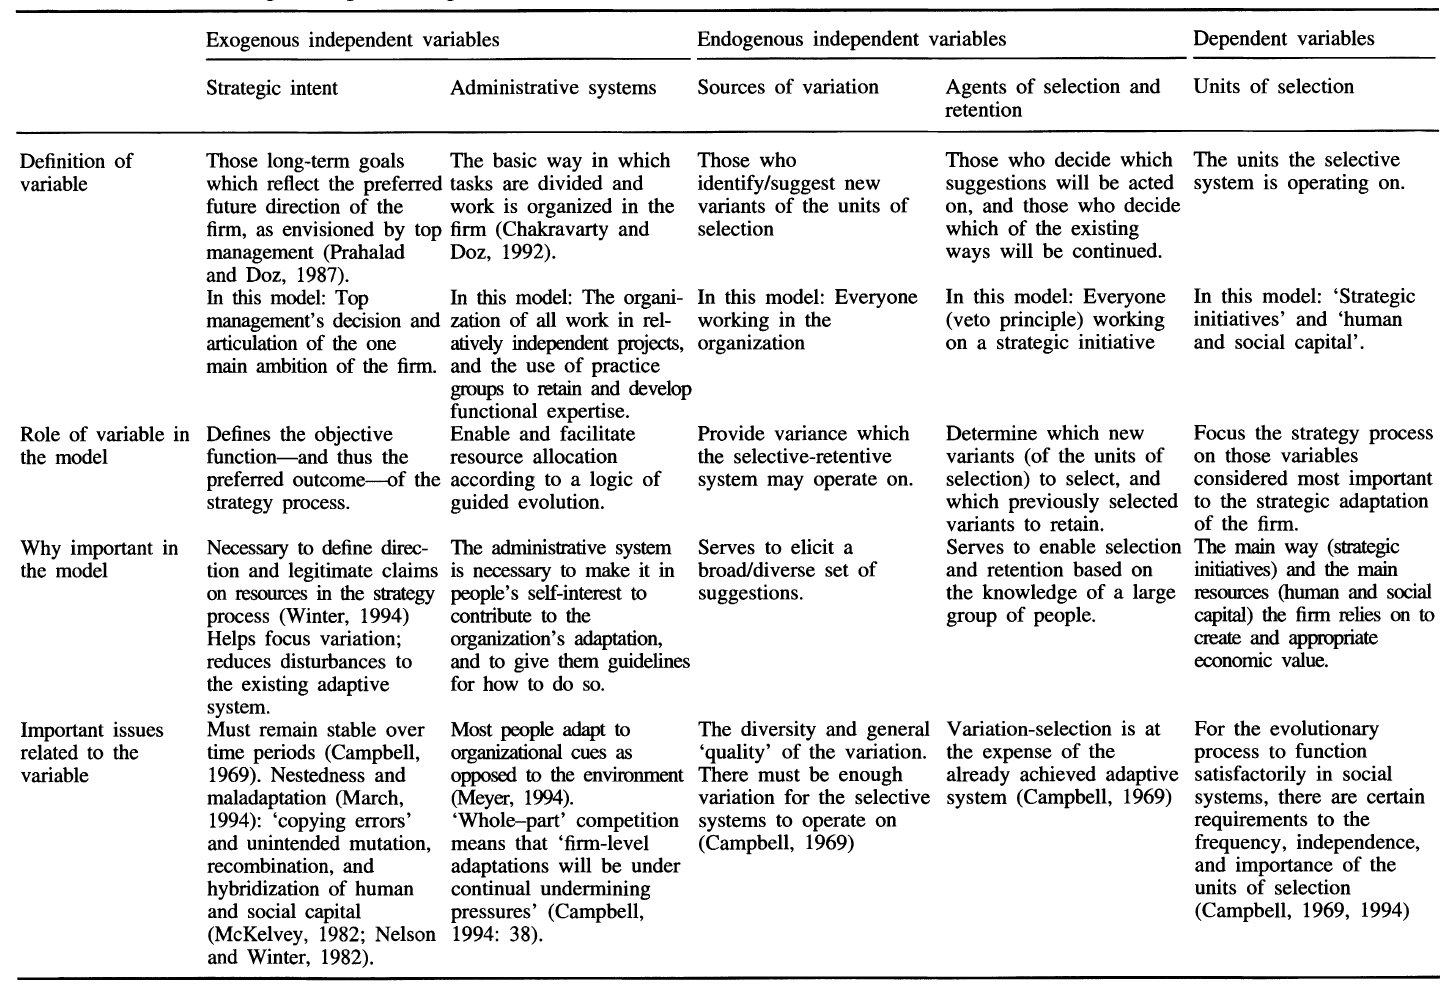
\includegraphics[width=\textwidth]{Lovas2000b}
  \label{fig:Lovas2000b}
\end{centering}
\end{figure}

\subsection{Applying on the  \cite{Lovas2000} model in a startup firm}
While all prior process theories discussed here focus their attention on traditional and typical large firms organized as hierarchies, I suggest here why they may remain quite relevant in the context of the entrepreneurial startup firm. First, the process theories lay their focus on the tasks of management, and it stands to reason that similar functions are performed in entrepreneurial firms even though not by a clearly designated management team. Second, the \cite{Lovas2000} model is particularly relevant to the startup firm because of the relaxing condition that all strategic initiatives maybe viewed as being either induced or as autonomous. This removes the requirement of a formal management team, and the concepts are now adaptable to the co-founding team that is traditionally vested with many of the functions of top management. Strategic initiatives may be induced in such a firm through a series of actions including those in recruitment,  financing and spinning off of independent projects. Finally, evolutionary models require that there be sufficient variance selective system to operate on, a condition mated well to startup firms. I therefore propose to build on top of the \cite{Lovas2000} model in presenting my research proposal.

\section{Research Proposal}
Scholars have highlighted that the central problem of evolution in cultural and social systems is the tension between the creation of new variants (new strategic initiatives) versus the retention of previously selected variants (existing strategic initiatives). This may be particularly salient in startup firms that are constrained on managerial experience or talent. I therefore pose the following question.

\subsection{Research Question}
How do founders in a startup firm simultaneously balance variation, selection and retention of ideas, people and projects over time in the pursuit of their strategic intent?

\subsection{Theory}
Strategic initiatives therefore 'emerge' pri- marily from managerial activities of front-line and middle managers, as implied by the Carnegie school bottom-up problem-solving perspective (Simon, 1945; Cyert and March, 1963; March and Simon, 1965) and suggested in many other descriptive strategy process studies. Nevertheless, top managers can exercise critical influences on these activities by setting up the structural context (i.e., various organizational and administrative mechanisms such as organizational architecture, information and measurement systems, and reward and punishing systems) to reflect the cor- porate objectives, and thereby manipulating the context in which the decisions and actions of lower-level managers are made (Bower, 1970), as suggested by the Harvard top-down administrative perspective (Chandler, 1962; Learned et al., 1965; Andrews, 1971). The development of those stra- tegic initiatives would lead to the refinement or change of the concept of corporate strategy, thereby determining 'strategic context' over time. Strategic context determination is conceived pri- marily as a political process through which middle managers delineate in concrete terms the content of new fields of business development for the corporation and attempt to convince top managers that the current concept of corporate strategy needs to be changed so as to accommo- date successful new business development (Burgelman, 1983a, 1983b).

The central feature of the B-B model is a resource allocation process in which bottom-up strategic initiatives compete for scarce corporate resources and top managers' attention to survive within the corporate contexts-structural and strategic contexts. Burgelman (1991), in his in-depth field study on Intel's corporate renewal, further developed the idea of intraorganizational competition among bottom-up initiatives and proposed an intraorganizational ecological perspective, fol- lowing the variation-selection-retention frame- work of cultural evolutionary theory (Campbell, 1969; Aldrich, 1979; Weick, 1979). Strategic initiatives are identified and examined in the definition process, within the corporate context (variation), are selected out in the impetus pro- cess by corporate context as 'internal selection environment' (selection), and lead to the reinforcement or modification of corporate context (retention). Burgelman (1994) argues that Intel's internal selection environment, particularly its 'maximizing margin-per-wafer-start' resource allocation rule, reflected selective pressures from the product market in ways that helped the firm exit from the increasingly competitive memory business and refocus on microprocessors.

\subsubsection{Leading into H1a}
We do so since the scale is symmetric across the Center (C), any initial mapping 
As March (1994) has noted, problem in attempting to 'engineer' or guide evolutionary processes in social systems is to specify what part of the system one is to optimize. This is a problem because social systems are nested in space; i.e., they consist of many different parts,
which are interrelated with one another. Because what might be best for one part of the system (e.g., the engineering department) may not be what is in the best interest of another part of the system (e.g., the marketing department), it is necessary to specify clearly what part of the system one wants to optimize on.
In the guided evolution model, the purpose of administrative systems is role. Its purpose is not to control the retention of predefined strategies, but to help manage the coevolution of strategic initiatives and human and social capital on a distributed basis. More specifically, the intention is to ensure that the variation, selection, and retention of strategic initiatives and human and social capital are informed by the local knowledge of people within the firm \citep{Lovas2000}. {Positive side in the role of management}
There are two important implications of such coevolution. On the positive side, to the extent top management can influence where and how employees use their time and energy, they can also influence what human and social capital is created and maintained. In the proposed model, this is done in two ways: first, by relying on a strategic intent to guide the evolution of strategic initiatives, thereby influencing the production and replication of the human and social capital that coevolve with them; and, second and related, by
relying on a strategic intent to signal what human and social capital top management expects to be valuable in the future, thereby influencing what skills, knowledge, and business relationships people are motivated to build and maintain \citep{Lovas2000}. 
\begin{hypothesis}
{Hypothesis 1a: When the institutional field is open to influence, slow learning adversarial agents will raise overall performance higher than slow learning agents with a neutral orientation\\}
\end{hypothesis}

\subsubsection{Leading into H2a}
source: \cite{Lovas2000} The members of the top management group had five main responsibilities: (1) to develop and articulate strategic goals which defined the strategic intent of the organization; (2) to sponsor strategic initiatives; (3) to allocate financial capital to strategic initiatives; (4) to recruit people to the organization; and (5) to take responsibility for the development of one area of functional expertise and knowledge in the organization. All employees who were not members of the top management group had two main responsibilities: (1) to work on at least two strategic initiatives at any given point of time; and (2) to have experience in two or more functional areas, in at least one of which he or she had to be an expert. In addition, some employees served as project managers, but then only as a temporary role for the duration of the project. {Negative side}
On the negative side, to the extent the strategic intent is not providing effective selection pressures in the internal ecological environment, the result may be random drift when undirected changes in the firm's stock of human and social capital accumulate from one time period to another (McKelvey, 1982; Hannan and Freeman, 1989). As a consequence, valuable human and social capital may be gradually lost. Likewise, if the strategic intent is changed, but does not guide the coevolution between strategic initiatives and
human and social capital in an adaptive direction, existing valuable human and social capital may be lost. Finally, if the strategic intent is changed too often, a firm may lose existing human and social capital through too frequent variation (e.g., mutation, recombination, hybridization), and not be able to focus long enough on a certain set of issues to develop and retain valuable human and social capital in any particular. 

\begin{hypothesis}
{Hypothesis 2a: For the same initial outcome preferences,  the overall performance score varies curvilinearly with difference in the rates of learning of the agent and the institutional field\\}
\end{hypothesis}


\subsection{Data and Method}
At around the turn of the century, PayPal found itself up against Billpoint. PayPal had been founded to enable secure digital payments between individuals, and had dedicated its strategic attention on its most important partner - eBay, an online auction marketplace. The vast majority of PayPal transactions at the time were happening on the eBay platform when eBay decided to partner with Wells Fargo Bank to launch its own payment system, Billpoint. PayPal faced competition from eBay (eBay would promote Billpoint to all its users) on its most valued platform. Yet, within a year PayPal triumphed over Billpoint and Ebay was forced into purchasing PayPay for \$ 1.5 billion in August 2002 (the deal completed in 2003).\par

The setting described above is characterized by the following attributes. First, PayPal and Billpoint were clearly direct competitors operating in the same industry and therefore subject to similar external environmental forces. Second, both PayPal and Billpoint were building a solution to the same problem. Third, both firms were located in the same region and had access to the same talent pool. Despite such similarities, and a presumable advantage (through the eBay parentage), Billpoint failed and PayPal succeeded. A comparative case study of the co-founder decision making process between the two firms, can potentially give us causal answers to what processes adopted at PayPal vis-a-vis that adopted at Billpoint specifically lead to PayPal\textquotesingle s success. The sample selection process described above is resilient to alternative explanations or endogenous factors to be proposed to weaken the findings. 
While it maybe argued that retrospective studies may suffer from survivor bias, I contend that this maybe adequately countered by relying primarily on archival data including internal memos, emails and press reports from the period that were describing process occurring at the time. 

Since neither PayPal nor Billpoint could have  possibly known upfront which strategic initiatives would lead to success, it stands to reason that the evolutionary response of PayPal co-founders to the problems at hand were superior to those of Billpoint. By inspecting founders\textquotesingle \ communications, hiring decisions, and sense giving processes, I expect to tease out the differences in the processes of simultaneously manipulating the conditions for variation, selection and retention of ideas, people and projects at each of the two competing firms. The rich data, coupled with the quasi-experimental setup will lead us to provide causal explanations for PayPal\textquotesingle s superior evolutionary and economic outcomes.

\section{Contribution}
Insights from the empirical study of the evolutionary processes in strategic initiatives at PayPal and Billpoint can potentially further the theory of strategy as guided evolution. In the least, I expect the study to add significant empirical insight to the processes of inducing strategic initiatives in startup firms.

\section{Summary}
In this paper, I have used the \cite{Lovas2000} model of strategy as guided evolution as an anchor to first review the literature on strategy process research, and then suggested a study that will apply the \cite{Lovas2000} to an empirical setting that promises to provide a causal inference of the sources of superior evolutionary approaches to the inducing of strategic initiatives. 



\begin{singlespace}
\renewcommand{\refname}{REFERENCES}
\bibliography{/Users/aiyenggar/code/bibliography/aiyenggar} 
\bibliographystyle{ai-amjlike}
\end{singlespace}

\newpage
\appendix
\begin{singlespace}
\section{APPENDIX A: Classical Process Models}
\begin{figure}[h]
\begin{centering}
  \caption{The Research Allocation Process, adopted from \cite{Bower1970}}
  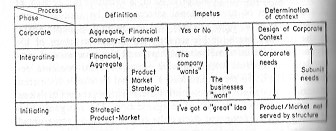
\includegraphics[width=0.85\textwidth]{Bower1970}
  \label{fig:Bower1970}
\end{centering}
\end{figure}

\begin{figure}[h]
\begin{centering}
  \caption{Types of Strategies, adopted from \cite{Mintzberg1978}}
  \includegraphics[width=\textwidth]{Mintzberg1978}
  \label{fig:Mintzberg1978}
\end{centering}
\end{figure}

\begin{figure}[h]
\begin{centering}
  \caption{Strategies form in subsystems (involving different people, skills, goals, information, and timing imperatives), adopted from \cite{Quinn1980}}
  \includegraphics[width=\textwidth]{Quinn1980a}
  \label{fig:Quinn1980a}
\end{centering}
\end{figure}

\begin{figure}[h]
\begin{centering}
  \caption{Some typical process steps in logical incrementalism (highly simplified to help visualize a few basic relationships), adopted from \cite{Quinn1980}}
  \includegraphics[width=\textwidth]{Quinn1980b}
  \label{fig:Quinn1980b}
\end{centering}
\end{figure}

\begin{figure}[h]
\begin{centering}
  \caption{Key and peripheral activities in a process model of ICV, adopted from \cite{Burgelman1983b}}
  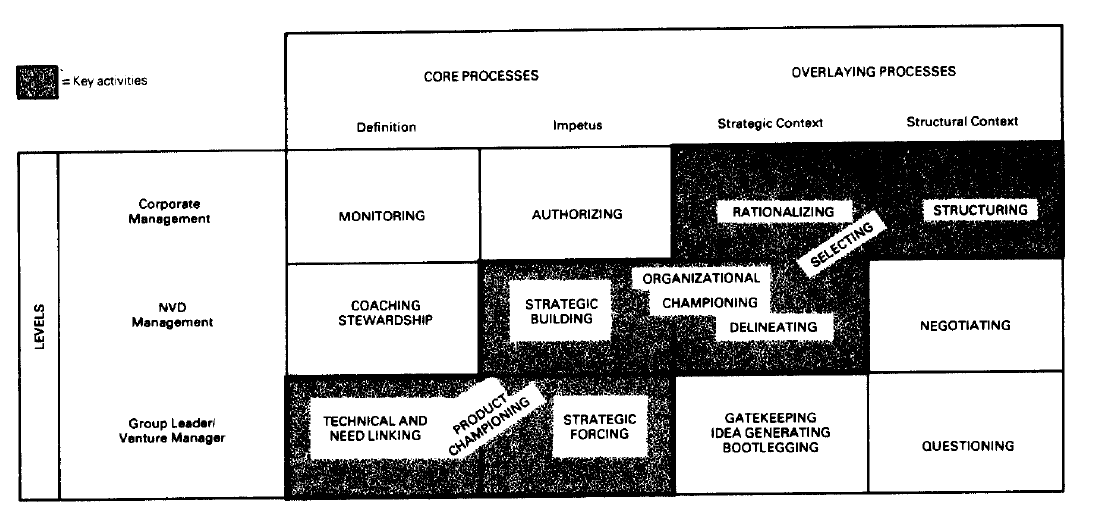
\includegraphics[width=\textwidth]{Burgelman1983b}
  \label{fig:Burgelman1983b}
\end{centering}
\end{figure}

\end{singlespace}

\end{document}
